\chapter{Kết quả nghiên cứu}

\section{Phương pháp tiếp cận}

\subsection{Sơ đồ khối hệ thống}

\begin{center}	
	\begin{figure} [ht]
		\begin{center}
			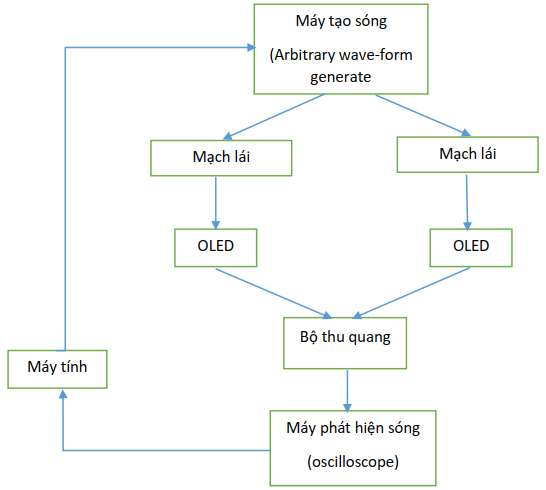
\includegraphics[width=0.5\textwidth,keepaspectratio]
			{sodokhoihethong.png}
		\end{center}
		\caption{Sơ đổ khối hệ thống MIMO-VLC} 
	\end{figure}
\end{center}


\textbf{a) TRANSMITTER}

Trong thập kỷ qua, ta đã chứng kiến sự sử dụng rộng rãi của diode phát quang (LED) trong rất nhiều ứng
dụng trong đời sống. LED đã chứng minh mình là một công nghệ mạnh mẽ cho lĩnh vực chiếu sáng, nhưng giờ
đây, ngoài khả năng chiếu sáng, khoảng băng tần khả kiến của LED còn có thể sử dụng cho truyền nhận dữ liệu
không dây, mà tại đó LED chính là nguồn phát dữ liệu. Bên cạnh LED, đèn LED hữu cơ (OLED) cũng đã là cơ sở
cho nhiều ứng dụng chiếu sáng và trình chiếu, đặc biệt là trong điện thoại di động hoặc các thiết bị cầm tay khác.
Việc này là nhờ vào công năng tuyệt vời của nó, như là kích thước nhỏ gọn, nhẹ, hình dáng có thể tùy chỉnh, tiêu
thụ ít công suất, chi phí sản xuất thấp.

Cả LED và OLED đều một lựa chọn rất được các nhà nghiên cứu quan tâm để dùng làm nguồn sáng cho
công nghệ VLC. Tuy nhiên, OLED lại có băng thông điều chế thấp hơn rất nhiều so với đèn LED thông thường.
Không giống như LED thông thường, OLED là tập hợp các phân tử hữu cơ, do đó độ linh động của nó thấp hơn
nhiều so với các thiết bị silicon khác, kết quả là sẽ giới hạn băng thông điều chế của nó. Băng thông điều chế của
OLED còn phụ thuộc vào nhiều thứ, như là quá trình sản xuất, kích cỡ,...nhưng băng thông thông thường của chúng
chỉ dừng lại ở vài trăm KHz.

Hình [3.1] mô tả đáp ứng tần số của OLED Lumiable sáng trắng tiêu chuẩn (do Philip sản xuất), có diện tích mặt phát quang là $4\pi cm^2$. Trong chiếu sáng và trang trí trên thị trường, đây là một trong số ít các OLED được bày bán. Các phép đo cho thấy băng thông điều chế của OLED này là khoảng 7kHz.


\begin{center}	
	\begin{figure} [ht]
		\begin{center}
			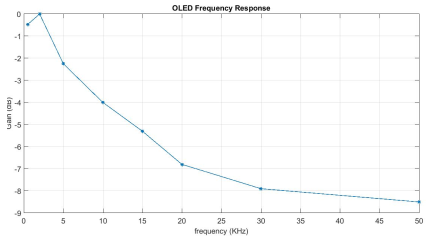
\includegraphics[width=0.5\textwidth,keepaspectratio]
			{dapungOLED.png}
		\end{center}
		\caption{Đáp ứng tần số của OLED} 
	\end{figure}
\end{center}

\textbf{b) RECEIVER}

Photodiode là một diode bán dẫn thực hiện biến đổi photon thành dòng điện theo hiệu ứng quang điện, các
photon có thể thuộc vùng phổ của ánh sáng khả kiến, hồng ngoại hay tử ngoại,...Photodiode sử dụng trong khảo
sát là APD410A do thorlab sản xuất, có thể thu được ánh sáng có bước sóng từ 400-1000 nm, băng thông 10MHz.

Các đặc tính cơ bản của bộ thu quang photodiode:

\begin{itemize}
\item Độ nhạy cao trong khoảng bước sóng hoạt động.
\item Thời gian đáp ứng nhanh, để thỏa mãn được các hệ thống có tốc độ cao.
\item Kết nối hiệu quả với cáp quang.
\item Đặc tính ít thay đổi theo nhiệt độ và thời gian sử dụng.
\item Tương thích với các thiết bị điện.
\item Chi phí thấp, độ tin tưởng cao.	
	
\end{itemize}

	\begin{center}	
	\begin{figure} [ht]
		\begin{center}
			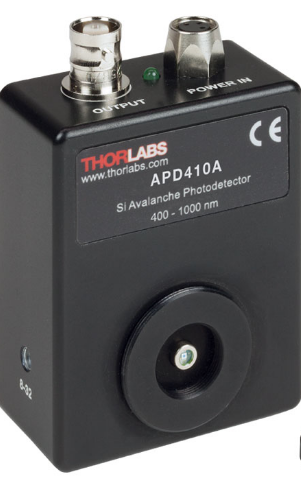
\includegraphics[width=0.25\textwidth,keepaspectratio]
			{photodiode.png}
		\end{center}
		\caption{Bộ thu quang APD410A của Thorlab} 
	\end{figure}
\end{center}

\subsection{Thí nghiệm 1}

Ở thí nghiệm đầu tiên, chúng em sẽ khảo sát và so sánh tỉ lệ lỗi bit ở các tốc độ bit khác nhau, sử dụng đồng thời 2 phương pháp ước lượng truyền thống và probabilistic neural network.

Các bước tiến hành thí nghiệm:

\textbf{Bước 1:} Tạo code tín hiệu NRZ từ máy tính bằng phần mềm matlab.Tín hiệu được tạo sẽ có chiều dài chuỗi bit, tốc độ lấy mẫu và biên độ ứng với các biến trong code.

\textbf{Bước 2:} Đưa tín hiệu vào máy tạo sóng. Có 2 điều cần lưu ý là phải giảm điện áp lái trên nguồn DC về 0 trước khi bấm nút "Output" để phát tín hiệu và ghi chú lại thời gian T trên đồ thị tín hiệu trên màn hình máy tạo sóng.

\textbf{Bước 3:} Kết nối dây từ nguồn DC,máy phát sóng và đèn \ac{oled} với mạch lái. Chú ý để mạch lái trên vật dụng bằng nhựa hoặc gỗ để tránh chạm mạch.

\textbf{Bước 4:} Bật nút "OUTPUT" trên máy tạo sóng, tăng điện áp nguồn lên dần dần.Quan sát thông số công suất trên màn hình DC và dừng tăng điện áp khi công suất đến ngưỡng 0.2 W-0.3 W. Nếu để công suất quá lớn sẽ làm cháy OLED do mạch lái OLED tạo các gai lớn.

\textbf{Bước 5:} Tín hiệu sau khi được thu qua photodiode sẽ hiển thị lên màn hình oscilloscope, lúc này ta cần chỉnh trục thời gian T'=2T để chắc chắn tín hiệu thu được chuỗi tín hiệu đầy đủ không bị mất. 

\textbf{Bước 6:} Sử dụng matlab để xử lý tín hiệu thu được và sau đó cho qua bộ neural network để khảo sát.

\textbf{Bước 7:} Lặp lại các bước như trên với các tốc độ bit khác nhau. Cách làm tổng quát sẽ là từ lý thuyết ta sẽ khảo sát ở tốc độ bit từ 50k đến 60k để tìm xem tỉ lệ lỗi bit sau khi đã sử lý qua neural network sẽ đạt ngưỡng ở tốc độ nào, sau đó ta sẽ tăng tốc độ hoặc giảm tốc độ rồi lấy dữ liệu để so sánh.

\subsection{Thí nghiệm 2}

Ở thí nghiệm này, ta sẽ so sánh tỉ lệ lỗi bit đã qua xứ lý neural network ở các khoảng cách khác nhau với cùng 1 tốc độ bit là 50kb/s. Các bước tiến hành như thí nghiệm 1 chỉ khác là ta sẽ giữ nguyên tốc độ bit và thay đổi khoảng cách.





 








